\documentclass{article}
\usepackage{xr}
\bibliographystyle{naturemag}
\renewcommand{\baselinestretch}{1.3} 
\usepackage{graphicx}



%% external tex files
%%\externaldocument{figure1_runtimes}
%%\externaldocument{figure2_powerFDRmultiple}
%%\externaldocument{figure3_mouse}

\externaldocument{supmaterials}

\begin{document}

\title{Eagle: Making multiple-locus association mapping on a genome-wide scale routine}
\author{Andrew W. George$^1$, Arunas Verbyla$^1$, Joshua Bowden$^2$}

\maketitle

%% To Add
%%-------------------------
%% 1. how real data were analysed



%%\begin{affiliations}
%%\item Data61, CSIRO, Australia.
%%\item IM \&T, CSIRO, Australia.
%%\end{affiliations}

\begin{abstract}

Methods for genome-wide association mapping have become progressively more sophisticated, statistically and computationally. Yet a well know limitation has persisted, the strength of association between a locus and trait is assessed only on a locus-by-locus basis. Statistically superior multiple-locus methods that detect multiple SNP-trait associations, simultaneously, have been available for some time but they have failed to become the method-of-choice. 
Here, we present Eagle for multiple-locus association mapping. Our goal was to develop a method that shifts mainstream association mapping from being single-locus to multiple-locus. We will show through the analysis of simulated and mouse data that Eagle finds true and avoids false 
associations better than completing single- and multiple-locus methods and does it faster. Eagle has been implemented as an R package, with a web-based Graphical User Interface (GUI) for users whom may be unfamiliar with R.
\end{abstract}


Over the past decade,  genome-wide association studies (GWASs) have changed considerably in both their analysis and design. Early studies
 followed a case-control design. Association mapping methods were no more complicated than contingency table tests or simple 
linear regression. These designs though had a tendency to yield spurious findings if there was unrecognised population stratification. This prompted a shift towards family-based designs and score tests, such as the tdt test and its variants (refs). Today, instead of by design, it is through statistical modelling that we account for the effects of population stratification (refs). This has meant that data can be collected from general populations, even if these populations are highly structured. Analysis via sophisticated association mapping methods, such as linear mixed model based approaches,  is now almost routine (refs).

What has not changed is that it remains common practice to analyse genome-wide association study (GWAS) data on a locus-by-locus basis. This is despite there being several significant problems with analysing data in this way. 
First, the aim of association mapping is to identify regions of the genome that house genes that are influencing a trait. 
The identification of these regions from these analyses is not always straightforward. GWAS results are reported, typically, via Manhattan plots 
that plot the -log$_{10}$ of the $p$ value for each locus against the map position of the locus. The $p$ valueue is obtained by testing the statistical 
significance of a SNP when treated as an effect in an appropriate model. 
The location of peaks in this plot identify genomic 
regions of interest. Inferring the exact number of regions though can be difficult if the peaks are not well separated. Second, when multiple statistical tests are performed, the probability of wrongly accepting a result (type 1 error) is inflated. This is known as the multiple testing problem (refs). Many different solutions have been offered (refs). Yet, there is still no well accepted way of correcting for multiple testing in the context of genome-wide association mapping. Third, many of the traits whose genetic secretes we are trying to discover are complex. There will be multiple SNPs in linkage disequilibrium with genes that are influencing the trait. Yet, a locus-by-locus mapping approach only assesses the evidence for association between a single marker locus and trait.

It is somewhat surprising then that multiple-locus association mapping methods haven't attracted more attention. Methods based on 
regularisation techniques, such as ridge regression (ref) and lasso (ref), measure all locus-trait associations simultaneously. 
Here, multiple testing is not an issue. These techniques though are computationally demanding. Also, their results can be difficult to interpret. The strength of association is not measured by a $p$ value but by the size of the regression coefficient for the SNP in the model. More recently, associations have started to be mapped with random forests (refs). Similar to regularisation techniques though, it is not clear how to infer genomic regions of interest from their findings (refs). A multiple-locus method that does show promise is the multiple-locus linear mixed model method (ref). The best multiple-locus model is built with simple forward selection. Results are immediately interpretable but here, computation becomes challenging for large datasets. 

In this paper, we present our new multiple-locus method for genome-wide association mapping, which we are calling Eagle. 
Eagle combines the strength of regularisation techniques (being able to fit all SNP-trait associations jointly), with forward selection giving easy-to-interpret threshold-free results.   We are able to achieve a computational performance similar to the fastest single-locus linear mixed model implementations 
through a dimension reduction step.
Our aim was to make multiple-locus association mapping on a genome-wide scale routine. To this end, we have implemented Eagle 
within an R package of the same name. 
Our package accepts marker data of different 
formats,  can handle data larger than a computer's  memory capacity, and makes heavy use of 
parallel computing for computation when available.  


\section{Results}

\subsection{Association Mapping Methods}

We compared Eagle, in terms of computational and statistical performance, against seven other association mapping methods. 
We chose methods that almost all had been purpose built for genome-wide analysis, that could handle data from quantitative traits, and where the methods had been implemented in freely available computer programs or packages. Two of the methods are based on single-locus (or locus-by-locus) models and five are based on multiple-locus models. Of the many ways of performing single-locus association mapping, we chose 
GEMMA \cite{zhou2012genome}  and FaST-LMM \cite{lippert2011fast} because of their popularity and computational speed. 
For multiple-locus association mapping, we chose bigRR \cite{shen2013novel}, glmnet \cite{Friedman2010glmnet}, 
LMM-Lasso \cite{rakitsch2013lasso}, MLMM \cite{segura2012efficient} , and r2VIM \cite{szymczak2016r2vim}.  
Each takes a different approach to multiple-locus association mapping. A summary of the key attributes of the different computer programs/packages 
is given in Supplementary Table \ref{suptabsummary} (See Methods for further details). 

 

\subsection{Simulation Study}
A large simulation study was performed where we sought to  answer two questions. 
First, how does Eagle compare, in terms of run time and memory usage, to 
competing implementations? Second, how well does Eagle find true associations (power) and avoid 
false associations (type 1 errors)? Data were generated under five different scenarios; a study of size 150 individuals 
and 5,000 single nucleotide polymorphisms (SNPs) (150 x 5K),  350 individuals and 400,000 SNPs (350 X 400K),  1,500 individuals and 
50,000 SNPs (1500 x 50K), 2,000 individuals and 500,000 SNPs (2000 x 500K), 4,000 individuals and 
1,500,000 SNPs (4000 x 1.5M), and 10,000 individuals and 1,500,000 SNPs (10000 x 1.5M).   
These scenarios reflect, at least in some cases, the sizes of study being performed in animals, plants, and humans.  

For each scenario, 100 replicates were generated. A single replicate consisted of SNP and quantitative trait data. 
Extra realism was introduced into the simulation study through the drawing of the SNP genotypes from the 1000 Genome Project, phase 3  \cite{10002010map}.
 The quantitative trait data were generated 
by selecting, randomly, a set of SNPs and assigning these loci additive allelic effects.  Random errors were then drawn from a normal distribution 
with variance set to give a heritability of 50\% for the trait. 
For each individual, a quantitative trait value was obtained by summing its random error and additive allelic effects. 
The number of randomly selected SNPs follows a Poisson distribution with mean 30. The size of the allelic effects 
 across the selected loci are equal.  

 
 %%=== Tense/flow  ==>>
 
 
 Analyses by the seven programs/packages of a replicate proceeded as follows. They were all run at their default settings. 
 Eagle and MLMM were the easiest of the programs/packages to implement. 
 The only parameters requiring specification were the amount of available memory and number of CPU for 
 Eagle and the number of chunks for MLMM. 
 Their results were also immediately 
 interpretable. Their findings were the set of SNPs in strongest association with the trait. Each 
SNP in this set identified a separate genomic region of interest, whose position was given by the map location of the SNP.  

BigRR, LMM-Lasso, and glmnet were not as easy to implement. They are based on regularisation methods and as such, all the SNPs were fitted simultaneously in a regression 
framework. The difficulty was in calculating the significance of the SNP effects. To do this analytically is challenging. We instead opted for stability selection (see Methods),  
an empirical approach for calculating significance. 

R2VIM is different from the rest in that it is a nonparametric approach for association mapping. It is based on random forests. Three important parameters needed to be  set. 
These were the number of trees, the number of variables for building a tree, and the minimum size of a terminal node. Ideally, these parameters would be "tuned" on a replicate-by-replicate 
basis (ref). However, this is not feasible here. We instead used the same settings as in \cite{szymczak2016r2vim} where 
the number of trees was set to 1000, the number of variables was set to 20\% of the number of SNPs, and 
  the minimum size of a node was set to 10\% of the sample size.
A relative importance measure was calculated 
for each SNP measuring its strength of association with the trait.

FaST-LMM and GEMMA implement single-locus association mapping. The $p$ values of the SNP were reported as their results. 


For all but Eagle and MLMM, the set of SNPs in strongest and significant association with the trait were found 
by placing the SNP in map order, setting a threshold, identifying peak regions with 
significance measures above the threshold, and recording the SNP with the largest significance measure in these peak regions. 


 
 



\subsection{Memory Usage and Run Times}

We analysed the simulated data with Eagle and the other computer programs, recording their memory usage and 
run (or elapse) times. The analyses were performed on a high-end desktop computer with dual 8-core Xeon processors and 128 gigabytes of RAM. Not all data generated under the five scenarios could be analysed by all implementations. Memory usage 
for many of the computer programs was the limiting factor (See {\bf Supplementary Figure \ref{supfigmem}}).  The single-locus program GEMMA was by 
far the most memory efficient. Not surprisingly, the multiple-locus programs were memory intensive. Most required in 
excess of the 128 gigabytes of available RAM for the analysis of data generated under 4000 x 1.5M and 10000 x 1.5M.  
Even FaST-LMM, a single-locus
implementation, required more than 128 gigabytes of memory for the analysis of the larger data sets 
when all the marker data was used to calculate the similarity matrix. Of the multiple-locus programs, only Eagle,  
with its ability to handle data larger than the memory capacity of the computer, was capable of producing findings 
for data from our largest scenario, 10000 x 1.5M. 


The median run times for Eagle and the other computer programs across the six scenarios are shown in Figure \ref{fig_time}. 
The x- and y-axes are on a log scale.  This means a unit change on the x- or y-axis is equivalent to a change in the order of magnitude.  In answer to our question of how does Eagle compare in terms of run time to competing implementations, 
Eagle was significantly faster, sometimes by orders of magnitude,  than the other multiple-locus
 implementations and is comparable to the single-locus implementations. For a simulation study with 150 individuals and 
 5000 SNPs, Eagle produced results in seconds.  For the larger simulation scenarios 1500 x  50K and 350 x4 00K, 
 analyses with Eagle took under two minutes. Even for data from a couple of thousand individuals and half a million 
 SNPs (2000 x 500K), the median run time of Eagle was under 14 minutes. For our scenarios where there 
 were thousands of individuals and 1.5 million SNPs, Eagle took just over two hours for the analysis of data from 
 4000 x 1.5M and  12 hours for the analysis of data from 10000 x 1.5M. 
 Towards the final stages of writing this paper, 
 we gained access to a desktop computer with 14-core Xeon processors with 256 gigabytes of RAM. We reran Eagle on data from the largest
  scenario 10000 x 1.5M to measure the impact on run time. The median run time dropped by more than 70\% 
  from 12 hours to 3.31 hours. 
 
  
 %%It is also worth noting that an increase in the number of SNP genotypes in a study does not necessitate, automatically,  
 %%an increase in the memory usage and run times for its analysis. This is  evidenced by the non-monotonically 
 %%increasing behaviour of the curves in the memory (Supplementary Figure \ref{supfigmem}) and run-time plots (Figure \ref{fig_time}).  It 
%%is the study dimensions, not number of genotypes, that drives the computing resources required by
%%association mapping programs.   

 
\begin{figure}
\caption{Median run times, in minutes, for the analysis of association study data from the six simulation scenarios. 
Eagle is compared against five other multiple-locus programs (top left plot) and two single-locus programs (top right plot). 
The x- and y-axes are on a log scale for improved aesthetics. Eagle has the lowest run-times of the multiple-locus 
programs, sometimes by orders of magnitude. Eagle can even produce results faster than single-locus programs. 
The actual median run times for the programs across the scenarios are given in the table. The entries in a bold font 
correspond to the lowest run-time for a scenario. 
 FaST-LMM$^{all}$ is where the single-locus results are based on all the available 
SNP data. FaST-LMM$^{few}$ is where the single-locus results as based on a subset of the available SNP data. }

\label{fig_time}
\begin{center}
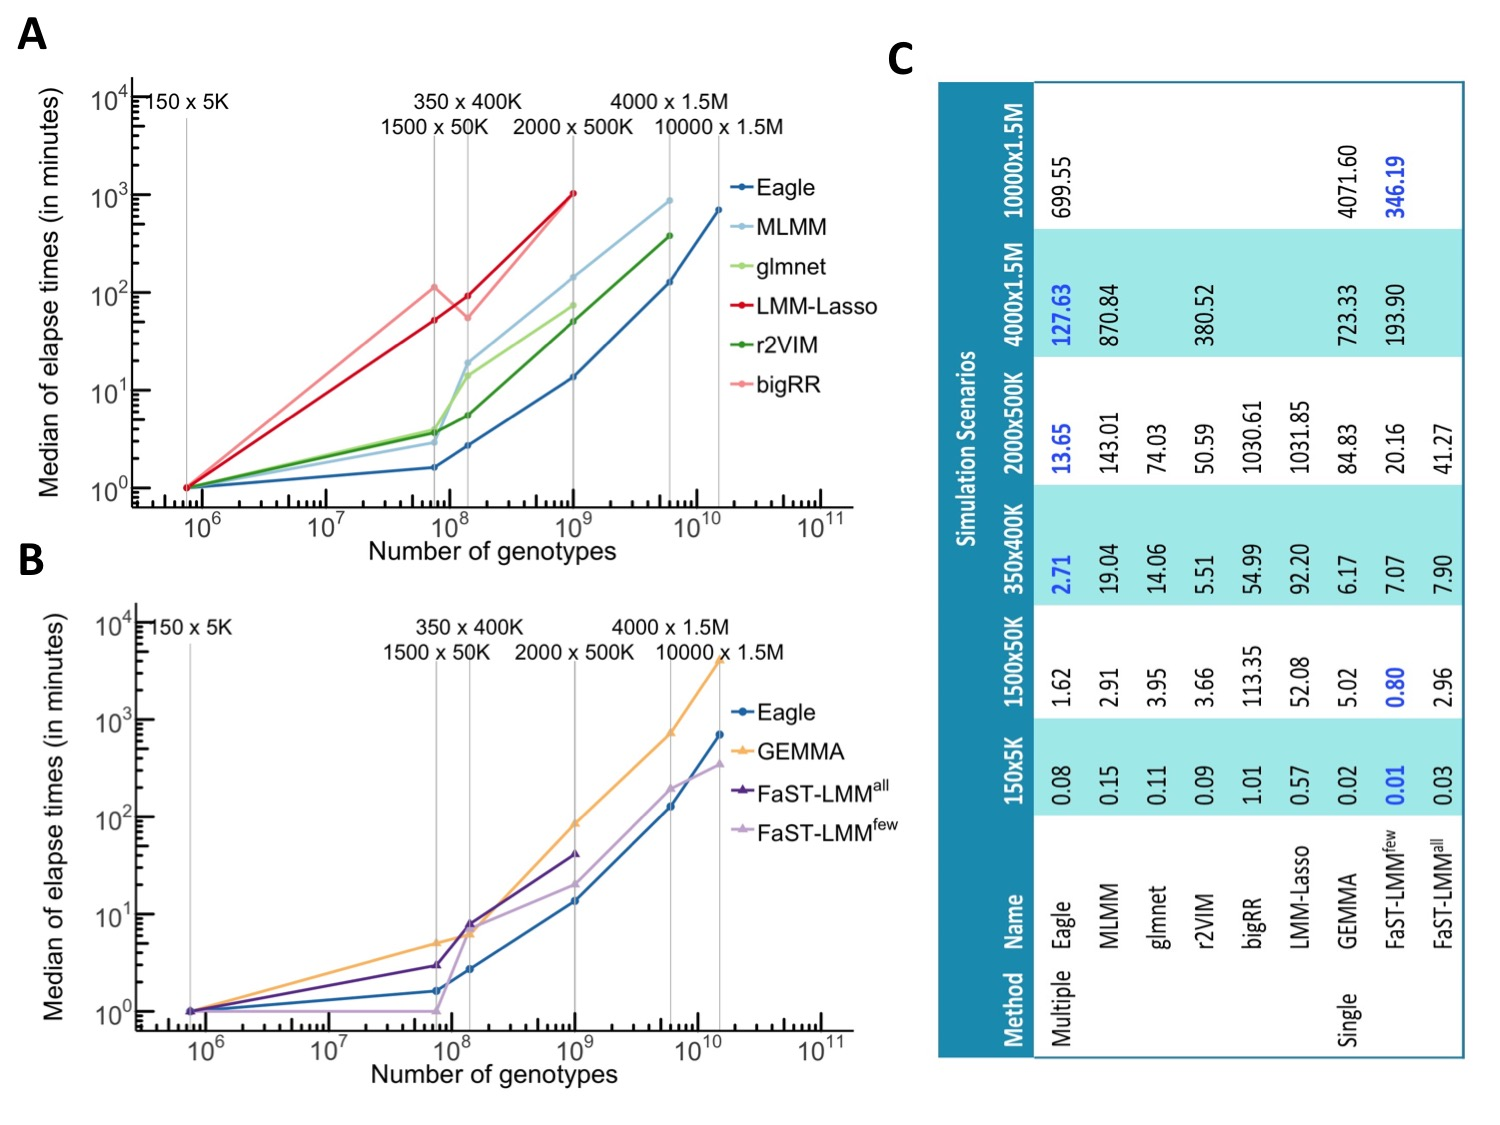
\includegraphics[width=18cm, height=14cm]{Figure2_time.jpg}
\end{center}

\end{figure}

 
 
%%{\em Figure \ref{fig_time} goes around here}





\subsection{Power and False Discovery Rates}

We calculated, empirically, the statistical power and false discovery rates of Eagle and the other methods across the six scenarios. 
We were interested in answering the question of how well Eagle finds true SNP-trait associations and avoids false SNP-trait associations. 
For each replicate, we knew which SNPs had been used in creating the quantitative trait data. These SNPs are in true association with 
the trait. It is the goal of the single- and multiple-locus association mapping methods to discover these SNPs. By knowing which SNPs are in true 
association with the trait, we were able to assess the validity of a  method's findings.  


To calculate the power of a method, for each replicate, we divided the number of true SNP findings by the number of SNP that had been used 
in creating the trait data. We then averaged across the 100 replicates.  
Similarly, to calculate the false discovery rate of a method, 
for each replicate, 
we divided the number of true SNP findings by the number of (true and false) SNP findings. We then averaged across the 100 replicates.  
A finding was counted as true if the SNP is located within 40 kilobase pairs of a SNP in true 
association with the trait. 


The power and false discovery rate of Eagle and the other multiple-locus methods across the scenarios 150 x 5K, 350 x 500K, 1500 x 50K, and 2000 x 500K are shown in Figure \ref{figpowermultiple}.  We restricted our attention to these scenarios for the multiple-locus methods because for scenario 4000 x 1.5M, 
the data could only be analysed by Eagle, MLMM, and r2VIM. For scenario 10000 x 1.5M, the data could only be analysed by Eagle. 
The power and false discovery rate of Eagle and the two single-locus methods, GEMMA and FaST-LMM,  are shown in
Supplementary Figure \ref{supfigpowersingle}.  Each plot contains 
single points and power curves. The single points are the power and false discovery rates for Eagle and MLMM.
These two methods treat association mapping as a model selection problem. Their are no significance thresholds to be set. 
The power curves are for those methods that treat association mapping as a parameter estimation problem. Here, the 
significance of the findings are assessed against a significance threshold. The power curves in the plot show how power changes with 
the false discovery rate as the significance threshold  is adjusted. 




\begin{figure}
\caption{Genome-wide association mapping results from the analysis of the mouse data for the single-locus method FaST-LMM and the 
multiple-locus method
Eagle. Eagle was run under two settings; its default setting (Eagle$^{default}$) and where the model selection criterion had been optimised 
for a false discovery rate of 5\% (Eagle$^{optimal}$). 
The number of SNP-trait associations found are reported. The bar plots with boxes around them are for those traits where using 
Eagle$^{default}$ and Eagle$^{optimal}$ resulted in more findings than with single-locus analysis.} 
\label{figmouse}
\begin{center}
%% obtained from bracewell by running ResultsV2.R from /data/geo047/MWAM/Mouse/OutBred/RScripts/
\includegraphics[width=15cm, height=15cm]{mouseresults.eps}
\end{center}

\end{figure}



%%{\em Figure \ref{figpowermultiple} goes here}


In answer to the question of how well Eagle finds true SNP-trait associations and avoids false SNP-trait associations, it does extremely 
well.  Of the multiple-locus methods, Eagle has the highest power
while keeping its false discovery rate low (Figure \ref{figpowermultiple}). MLMM also performed well. However, it is when Eagle is compared against single-locus methods 
that the difference in power is most noticeable.  Eagle has much greater power than single-locus methods for finding SNP in true 
association with a trait while avoiding false associations (Supplementary Figure \ref{supfigpowersingle}). 



%%At first glance, Eagle appears underpowered. Several of the other methods have higher power than Eagle. The goal of association mapping though is not only to find true SNP-trait associations but to also avoid false SNP-trait associations. For those methods with higher power than Eagle, the cost is much higher false discovery rates. In other words, these methods are finding more true results  but they are also finding many more false results. If we restrict our attention to that part of the plot where the (genome-wide) fdr is less than  5\% (see inset plots in Figure X and Sup Figure X),  we see that Eagle, closely followed by MLMM,  has the highest power for the lowest  fdr. This is especially true when the power and fdr of Eagle is compared to the single-locus methods. For single-locus methods to achieve the same level of power as Eagle, a threshold has to be set where the fdr is extremely high. 



\begin{figure}
\caption{Power verse false discovery rates for Eagle and the multiple-locus methods. Plots for only those simulation 
scenarios where all multiple-locus methods could be implemented are shown.  Eagle has the highest power across the four 
scenarios but MLMM also performs well. }
\label{figpowermultiple}
\begin{center}
\includegraphics[width=15cm, height=15cm]{power1main.eps}
\end{center}

\end{figure}


%% {\em Figure \ref{figpowermultiple} goes here}



\subsection{Mouse Data Analysis}

We were interested in comparing results from Eagle with those from single-locus association mapping for a real data set.
 We chose to focus on data from a large outbred mouse study \cite{nicod2016genome}. This study was unusual in that it collected and analysed SNP dosages (continuous values from zero to one of expected allele counts)  instead of the more common SNP genotypes. Analyses based on dosages rather than discrete genotypes have been shown to have greater power for the detection of genes that are influencing a trait  \cite{zheng2011comparison}. By converting the dosages into genotypes and analysing the data with the single-locus program FaST-LMM, we obtained a subset of those findings reported in the original study. We then analysed the data with Eagle. Due to Eagles increased power, we found SNP-trait associations not found with the FaST-LMM. However, we were 
 able to confirm the validity of these new findings as they matched what was found in the original study. Having the ability to confirm new findings 
 in a real study was 
 one of the primary motivators for choosing these data for analysis. 
For the single-locus analysis of the data, we followed the same procedure as originally followed for the analysis of the mouse data \cite{nicod2016genome}. The only differences were that we focused on the autosomal SNP and it was necessary to 
increase the number of permutations for the controlling of the false discovery rate from 100 to 500.

Eagle was run in two ways; under its default settings (Eagle$^{default}$) and where we specified the regularisation parameter for model selection (Eagle$^{optimal}$ ) Eagle chooses the best model via the extended Bayesian information criteria (extBIC) \cite{chen2008extended}. 
  The conservativeness of the extBIC can be adjusted by a single regularisation parameter that ranges from zero to one. In the simulation study, this parameter was set to one, its most conservative and default setting. However, there is also opportunity to set the parameter to a value less than one. This increases power but also increases the false discovery rate. For each trait, we used permutation to set the regularisation parameter to give a false discovery rate of 5\% .

The genome wide results from the analyses of the mouse data are shown in Figure  \ref{figmouse}. The mouse study took
measurements on 200 traits. When these traits were first analysed in the original study, findings for 45 of these traits were able to be 
corroborated by prior published evidence. We focused our analyses here on these same 45 traits. For 39 traits, we found SNP-trait associations. 
For the other six, neither FaST-LMM nor Eagle found any associations. 
Each plot contains the number of SNP-trait associations that were found and in agreement with the original findings. 
Neither method found SNP not identified in the original mouse study so neither method found false positives. 
As we saw in the simulation study, there is a notable difference in the two methods capacity to discover SNP-trait associations. Eagle$^{default}$, under its default settings, for eight traits found the same number of findings as FaST-LMM and for 28 traits found more findings. Eagle$^{optimal}$, 
with its regularisation parameter fine tuned to the trait, for six traits found the same number of findings as FaST-LMM and for 32 traits 
found more findings. Overall, FaST-LMM, Eagle$^{default}$, and Eagle$^{optimal}$ found 26, 65, and 95, snp-trait findings respectively. 
Eagle$^{default}$ and Eagle$^{optimal}$ found two-and-a-half times and over three-and-a-half times, respectively, more SNP-trait 
associations than what is the established way of analysing these data. Furthermore, these are all findings that were confirmed in the original study. 



\section{Methods}


\subsection{Mouse Data}

The data were obtained from a large genome-wide association study which was performed in outbred mice \cite{nicod2016genome}. 
Phenotypic and genotypic data were available on 1,887 adult mice. 
The phenotypic data consisted of measurements from 200 behavioural, tissue, and physiological traits.  Of these traits, 
43 yielded SNP-trait associations that could be corroborated through other independent published work. It was these 
43 traits that were the focus of our real data analyses. Genotypic data were available on 359, 559 (353,697 autosomal) SNPs in the 
form of marker dosages (expected allele counts that ranged from zero to one). All missing data had been imputed. 
We converted the dosages into discrete genotypes 
by clustering around 0, 0.5, and 1, corresponding to SNP genotypes AA, AB, and BB, respectively. 


\subsection{Eagle Approach for Multiple-locus Association Mapping}

Eagle is a method for multiple-locus association mapping on a genome-wide scale. It is based on linear mixed models. It differs from most other single- and multiple-locus association mapping methods. Eagle treats association mapping as a model selection instead of variable selection problem. Consequently,  we do not have to contend with multiple testing issues or having to construct significance thresholds.  
Eagle also 
reports as its findings only those SNPs that are in strongest linkage disequilibrium, and hence closest, to the genes influencing a trait. 
The methodological foundation for Eagle comes from a whole-genome linkage analysis method that was developed for mapping 
quantitative trait loci in experimental crosses \cite{verbyla2007analysis} 


Let $S = \{ S_1, S_2, \ldots, S_s\}$ be a set of ordinal numbers where $S_k$ is the $S_k$th ordered SNP that was 
selected in the $k$th iteration. Suppose three iterations of our model building procedure 
have been performed and say the 500023rd, 15th, and 420th, 
SNP were selected, then $S=\{500023, 15, 420\}$. 
Let $y^{(n \; \times \;1)}$ be a vector containing $n$ measurements of the quantitative trait. 
Let $M^{(n_g \; \times \; L)} = [m_1 m_2 \ldots m_L]$ be a matrix containing the genotype data which have been collected 
from $L$ loci that span the genome on $n_g$ groups/lines/strains.  Here, $n \geq n_g$ meaning that a single or several trait measurements 
may be taken of the same group/line/strain. 
 It is common for the columns of $M$ to be in map order but this is not a requirement. 
The vector $m_j^{(n_g \; \times \; 1)}$ contains the genotypes for the $j$th SNP. 
The genotypes are coded as -1, 0, and 1 corresponding to SNP genotypes AA, AB, and BB, respectively. 

The specifics of the Eagle method are as follows. 
Eagle builds the "best" model iteratively, via forward selection. 
Suppose $s$ iterations of our model building process have already been performed. This means $s$ SNP-trait 
associations have been identified.  It also means that $s$ separate genomic regions of interest have been found.  
To perform the $s+1$th  iteration, we first fit the current model to the data. 
The (current) model is of the form 
\begin{equation}
\label{eq1}
y = X \tau + Z u_g + e
\end{equation}
where 
$X^{(n \; \times \; p)}$ and $Z^{( n \; \times \; n_g)}$ are known design matrices with $X$ being of full rank and $Z$ 
containing zeros and ones that assign the appropriate genetic effect to each measurement. 
The vector 
$\tau^{(p \; \times \; 1)}$ has $p$ fixed effects parameters including the intercept. The vector 
$u_g^{(n_g \; \times \; 1)}$ contains the 
genetic effects. The vector of residuals is 
$e^{(n \; \times \;1)}$ whose distribution is assumed to follow $N(0, \sigma^2_e I^{(n \; \times \; n)})$. 
So far,  this model differs little from standard linear mixed models for association mapping (refs). 
However, 
it is how we specify $u_g$ that distinguishes our model from others. 

The genetic effects $u_g$ are modelled as 
\begin{equation}
\label{eq2}
u_g = \sum_{k=1}^s  m_{S_k} a_{S_k} + M_{-S} a_{-S}
\end{equation}
where $m_{S_k}^{(n_g \; \times \; 1)}$ is the vector of genotypes for the $S_k$th SNP locus which is the $k$th selected SNP, 
$a_{S_k}$ is the additive effect of the $S_k$th SNP locus, $M_{-S}^{(b \; \times \; L-s)}$ is the matrix of  SNP genotypes 
with the data for the selected SNP in $S$ removed,  and $a_{-S}^{(L-s \; \times  \; 1)}$ is a random effect whose distribution is 
$a_{-S} \sim N(0, \sigma_a^2 I^{(L-s \; \times \;  L-s)})$. 
The terms in the summation on the left hand side are fixed effects.  The other term is a random effect.  The terms 
in the summation account 
for the additive effects of the selected snp that are in linkage disequilibrium with genes that are influencing the trait. The other term models 
snp-trait associations along the entire genome, simultaneously, except for those snp that have already been selected. 
This is a simple genetic model but it 
is effective for discovering snp-trait associations. 


Second, we estimate the parameters of (\ref{eq1}) and (\ref{eq2}) via residual maximum likelihood estimation. 

Third, we identify the $(s+1)$th snp that is in strongest association with the trait, based on the maximum score statistic
$t_j^2 = \frac{ \widetilde{a} _j^2}{\textrm{var}(\widetilde{a}_j)}$ where $\widetilde{a}_j$ is the best linear unbiased predictor (BLUP), 
and $\textrm{var}(\widetilde{a}_j)$ is its variance. This statistic is not only appealing intuitively, where we 
identify a snp based on its (random) effect size and accuracy, but is theoretically justified.  It follows from outlier detection 
in linear and linear mixed models (ref). 

Fourth, we determine the importance of the $(s+1)$th selected snp via a model selection strategy. 
We begin by reforming (\ref{eq2}) where $S$ now contains the $s + 1$ selected snp.  We then fit this new model to the data
via maximum likelihood and calculate its extended Bayesian information criteria (extBIC) \cite{chen2008extended}.  The 
extBIC is a model selection measure that takes into account the number of unknown parameters and the complexity 
of the model space.  It is especially well suited to the model selection problem in genome-wide association studies \cite{chen2008extended}. If this new model has a larger  than the current model, then the $s+1$th selected snp is added to 
the current model and the above process is repeated. If this new model has a smaller extBIC than the current model, then the 
model building process is complete. The set of snp in strongest association with the trait is the $s$ snp previously identified. 

\subsubsection{Reducing the dimension of the model}
In practice, estimating the parameters of (\ref{eq2}) can be demanding, computationally. 
The vector $a_{-S}$ has $L-s$ random effects where in modern genome-wide association studies, 
$L$, the number of snp, can be extremely large.  An alternative model is given by 
Verbyla \cite{verbyla2012rwgaim,verbyla2014whole}. 
They show how to reformulate (\ref{eq2}) to be a model with a random effect with only $n$ elements
\begin{equation}
\label{eq3}
u_g = \sum_{k=1}^s  m_{S_k} a_{S_k} + (M_{-S} M_{-S}^T)^{1/2} a^*_{-S}
\end{equation}
where $a^* \sim N(0, \sigma_a^2 I^{(n_g \; \times \;  n_g)})$, and 
$(M_{-S} M_{-S}^T)^{1/2}$ can be calculated via single value decomposition (ref).  
Although it may not be obvious, the two models are equivalent, 
having identical variance structures. Yet, the computational cost of model (\ref{eq3}) compared to 
model (\ref{eq2}) is much less, due to the random term in model (\ref{eq3}) having only $n$ instead of $L-s$ 
effects needing estimating. 

Verbyla \cite{verbyla2012rwgaim,verbyla2014whole} go on to show how to recover $\widetilde{a}$ from estimates from model  (\ref{eq3})  with 
\begin{equation}
\widetilde{a} = \left [ M_{-S}^T (M_{-S} M_{-S}^T)^{-1/2} \right ] \widetilde{a}^*
\end{equation}
where its variance matrix is
\begin{equation}
\label{eq4}
\textrm{var}(\widetilde{a}) = M_{-S}^T (M_{-S} M_{-S}^T)^{-1/2} \textrm{var}(\widetilde{a}^*) (M_{-S} M_{-S}^T)^{-1/2} M_{-S}
\end{equation}
These values are needed in order to calculate the score statistic $t_j^2$ for identifying the snp in strongest association with the trait. 
Fortunately, when calculating $t_j^2$, only the diagonal elements of the variance matrix are needed which simplifies the  calculation. 
of (\ref{eq4}). 



\subsection{Comparison Methods}

\subsubsection{Multiple-locus methods}

We compared the computational and statistical performance of Eagle against five other multiple-locus methods for 
association mapping  These were BigRR, LMM-Lasso, glmnet, MLMM  and, r2VIM. 
These five methods were selected because of their demonstrated value 
for analysing genetic data, they reflect a range of different statistical methodologies for association mapping, and they are available as 
either stand-alone computer programs or as  packages.

BigRR, LMM-Lasso, and glmnet  implement three different regression-based regularisation methods; generalized ridge regression, 
lasso, and elastic net, respectively. Regularisation methods can handle parameter estimation problems where the number of predictors is
 far greater than the number of  samples. This is made possible through a penalty function that balances bias against variance. 
The application of regularisation methods to association mapping has appeal because it means that the snp effects across an 
entire genome can be estimated, simultaneously. 
All three methods are sophisticated pieces of statistical machinery but the significance of an effect, which 
is needed in association mapping,  can not be calculated easily. Permutation has been suggest as an empirical solution to this 
limitation \cite{shen2013novel} 
but we have instead opted for stability selection (see below).

MLMM, of the five multiple-locus methods, is the closest in philosophy to Eagle. It too is based on  building the 
best  linear mixed model via forward selection using the ExtBIC criterion. 
However, there are several differences between the two methods.
 MLMM does not make use of dimension reduction and they are implemented quite differently leading to substantial 
 differences  in run time and memory usage (see Results).  Also, they differ in how a model is built. 
 Eagle uses a score statistic formed from parameter estimates of the random genetic effect in which to identify the next snp to enter 
 the model.  MLMM uses the statistical significance of a snp when it is treated as a fixed effect in the model. 
 This necessitates fitting a separate linear mixed model for each unidentified snp. Fortunately,  MLMM does do this 
 efficiently.
 
R2VIM is quite different to the other four methods. Here, a non-parametric model-free rather than model-based statistical approach is adopted. 
R2VIM implements random forests and a new way of measuring the importance of a snp.  
In random forests, the worth of a predictor is measured, empirically, by calculating its importance score. 
It is from these importance scores that snp can be ordered in terms of their strength of association with a trait. 
The difficulty is in knowing what proportion of the 
highest ordered snp are in true association. R2VIM addresses this by performing multiple parallel runs. Each run uses a different 
random seed, giving slightly different results for the random forest analyses. Within a run, a relative importance score (f) is calculated for 
each snp. The greater f is than one, the more evidence there is that the snp is in association with a trait.  A snp-trait association is 
declared if f for the snp is above some threshold value across all parallel runs. The difficulty is that the relationship between 
this threshold value and the chance of finding false positives is unknown.  The threshold value could be found via permutation but 
this would be computationally challenging for all but the smallest of association studies. 


\subsubsection{Single-locus methods}

We were also interested in comparing Eagle to single-locus methods to measure the difference in run times and statistical power. Even by limiting our focus to LMM-based methods, there were a number of efficient applications to choose from. 
We decided on GEMMA \cite{zhou2012genome} and FaST-LMM \cite{lippert2011fast}. These two applications have the same computational complexity \cite{zhou2012genome}, produce exact instead of approximate results, and are highly efficient computationally. They were developed at the same time, independently, but are similar theoretically. Both perform a single spectral decomposition of the relationship matrix $K$. Both use the eigenvector matrix to rotate the data. Both reformulate the log likelihood and 
restricted/residual maximum-likelihood (REML) 
log likelihood into a sum of $n$ terms that are easier to compute. The difference lies in their estimation procedure. FaST-LMM implement's the Brent's algorithm to optimise $\delta$. GEMMA instead implement's the Newton-Raphson algorithm. Newton-Raphson is more complicated in that it also requires the first and second derivatives of a function to be calculated. However, it is superior in terms of its convergence properties to the Brent algorithm.  Both applications are stand-alone computer programs, popular, and in common use.


\subsection{Stability Selection}
When using BigRR, LMM-Lasso, and glmnet, the results are affected by the amount of regularization ($\lambda$). 
BigRR has an approximate way of setting each snp's separate regularization parameter (ref). However, the optimal value of 
$\lambda$ must be found when using LMM-Lasso and glmnet. Also, 
all three applications yield the effect sizes of the snp across the entire genome but not their statistical significance. To address 
these issues, we made use of stability selection \cite{meinshausen2010stability}. 
Stability selection is a resampling strategy.  With stability selection, we were able to avoid having to optimise $\lambda$ while 
still being able to calculate, empirically, the statistical significance of the snp effects.

We performed stability selection as follows. For LMM-Lasso and glmnet, we performed a preliminary analysis to find an 
appropriate value for the regularization parameter.  We adjusted $\lambda$ so that LMM-Lasso and glmnet yielded 
between 10 to 30 snp with non-zero effects. Fortunately, with stability selection, the setting of $\lambda$ does not have to be exact 
 We then repeatedly subsampled, 
without replacement, the data. As recommended \cite{meinshausen2010stability}, we draw 100 subsamples of size $n/2$. We 
analysed the subsample, with $\lambda$ fixed for LMM-Lasso and glmnet.  To calculate, empirically,  the statistical significance of each 
SNP across the genome, we counted the number of times a SNP had a non-zero effect size over all the replicates. We then 
divided this number by the number of replicates (which was 100) to form an empirical probability estimate of the significance of a SNP. 


For BigRR, we modified our stability selection procedure slightly. 
There was no need to find an appropriate value for the regularization 
parameters as the BigRR package has an internal procedure for their 
calculation. We draw subsamples as above and analyzed the data with BigRR. However, within an analysis, we ordered 
the SNPs according to the absolute size of their SNP effects and recorded the top 20 SNPs. We then measured the significance 
of the SNPs across the entire genome as above. 



\subsection{Generation of Simulation Data}

The data were generated via data perturbation (Zhao et al. 2007). Data perturbation amalgamates real with simulated data to generate replicates. 
It is a way of introducing greater realism into a simulation study. 
 Here, the genotype data are real, the 
quantitative trait data are simulated. 
 The SNP genotypes were drawn, 
according to the specifications of the scenario, from data collected from the 1000 Genome Project, version 3   \cite{10002010map}. 
Across scenarios, the SNP data differs. Across replicates within a scenario, the SNP data are the same. 

To generate the trait data $y$, first, $q$, the number of SNP that are to be assigned a quantitative value is drawn from a Poisson distribution with 
mean 30. Second, $q$ SNP are selected randomly. Third, we assume an additive model for the SNP. The SNP genotypes AA, AB, and BB 
are assigned the values -1, 0, and 1, respectively. Fourth, the SNP effects are summed across the $q$ selected loci, for each individual, to 
generate a $g^{(n \times 1)}$ vector of genetic values where $n$ is the number of individuals. 
Fifth, $e^{(n \times 1)}$, a vector of residuals, is drawn from a normal distribution where $e_i \sim N(0, \sigma^2_e)$ and $\sigma^2_e$ is 
the residual variance that has been set to yield a trait with heritability 0.5. Sixth,  the trait data are formed as $y =  g + e$.  
In forming $y$, we have purposely not included any other environmental variables such as age, sex, or experimental design effects. This is because 
not all the methods were implemented to handle the inclusion of additional fixed effects. A two-stage modelling approach (ref) 
is often adopted to deal with this situation, be we chose not to introduce this complexity to the analyses.  


\subsection{Analyses of Mouse Data}




\subsection{Implementation}

Eagle has been implemented as an R package of the same name. Much of the heavy computation though is performed outside of R 
via C++ functions that utilise Eigen C++ routines. Eagle has been purpose built to rely heavily on calls to BLAS and LAPACK, 
mathematical libraries common to most computer systems. By making use of multi-threaded  BLAS and LAPACK libraries, many of the 
calculations in Eagle are parallelised. We have gone to great lengths to make Eagle easy-to-use. Tutorials, videos, How-To guides, and 
a link to our server for demonstrating Eagle on some test data are available on the Eagle website (ref).  
Eagle is available for download from the CRAN website. 

  
  
\section{Discussion}
Eagle is a new linear mixed model based method (and R package) for multiple-locus association mapping. It advances the state of association mapping in several ways. 
First, its computational footprint is much smaller than other multiple-locus implementations. Eagle makes multiple-locus analysis 
practical, even when the datasets are large. Second, the results from
 Eagle are immediately interpretable. They are the set of SNPs in strongest association with the trait where 
each SNP identifies a separate genomic region of interest. Third, it treats association mapping as a model selection problem, avoiding 
multiple testing issues and the need for significance thresholds. 
 As we saw in the simulation study, Eagle has considerably higher power than single-locus methods but is comparable in run time.
Also, when analysing the mouse data, Eagle found more than double the SNP-trait associations than 
with single-locus association mapping, the method of choice. Furthermore, these extra findings were all true. 

Eagle outperformed the other multiple-locus methods in our simulation study. However, we are aware/cognisant that we made several implementation 
choices that impacts our conclusions.  For instance, we chose to calculate the significance of the 
SNP effects from bigRR, LMM-Lasso, and glmnet via stability selection.  Permutation (ref) and multi sample-splitting (ref) are also equally valid empirical approaches. Stability selection though has the advantage of being based on repeated sampling of only a proportion (50\% in our case) of the 
data. Also, when analysing the (sub)samples, it was not necessary to calculate the entire solution path for a method. 
 Instead,  analyses are 
performed for a fixed value of the regularisation parameter, greatly reducing the amount of computation required. For r2VIM, an R package 
implementing random forests, we had to decide on the  minimum size of a terminal node, the number of trees, and number of potential variables. 
The setting of these parameters greatly affects performance.  We  acknowledge that in the hands of an expert, 
r2VIM could of been fine-tuned for a better balance of computational and statistical performance because random forests are highly adjustable. 
However, we would like to think that the parameter settings we used are sensible since they match the values in the original r2VIM publication (ref). 

Eagle's computational speed does come at a cost. It is a weakness shared by all of the methods considered here, although in different ways. 
Eagle cannot handle extra random effects which are sometimes needed when more advanced study designs are employed. One solution 
is to adopt a two-stage analysis procedure. In the first stage, a single linear mixed model is fitted to the data. Much of the modelling complexity, 
including the extra random effects, is 
captured in this first-stage model. In the second stage, Eagle is run not on the original but adjusted trait data which were obtained from the first stage analysis. Even though this is a well accepted practice, it is approximate (ref).  A better solution is to fit a single model to the data. 
Although not specifically designed for association mapping,
WGAIM, upon which Eagle is based, and RRGAIM are two R packages where this is possible. Here, the difficulty is that for large datasets and/or complex 
models,  run time and memory usage can become limiting factors for analysis. 


Over the coming years, computationally, the demand placed on association mapping methods is going to increase. 
High-throughput array-based technologies continue to decrease the cost of genotyping, permitting ever larger GWASs to be performed. 
Whole-genome sequencing is also now a reality. Already sequence across entire genomes are being collected for GWASs (refs), 
culminating in data on millions of SNPs. It is because of this growing demand that 
we have purposely structured the Eagle package for continued development. We are already experimenting with a GPU-based version of Eagle. 
Early results suggest that for small to moderate sized datasets (<10,000 samples), there is little improvement in performance over CPU-based 
computation.  However, for larger study sizes, we are seeing up to a 40\% decrease in run times.  
We also have plans for Eagle to run on computer clusters. Structuring Eagle for larger-than-memory calculations was a 
preemptive step in this direction. GWASs have changed significantly in the past decade but the size and complexity of GWASs is expected 
to change even more in the coming decade. 




















%%\bibliographystyle{naturemag}
\bibliography{biblibrary}


%%\begin{addendum}
%% \item Put acknowledgements here.
%% \item[Competing Interests] The authors declare that they have no
%%competing financial interests.
%% \item[Correspondence] Correspondence and requests for materials
%%should be addressed to A.B.C.~(email: myaddress@nowhere.edu).
%%\end{addendum}



\end{document}
